\documentclass[solution,addpoints,12pt]{exam}
\printanswers
\usepackage{amsmath,amssymb,graphicx}
\usepackage{centernot}
\usepackage{hyperref}
\newcommand{\RP}{\ensuremath{\mathsf{RP}}}
\newcommand{\expect}[1]{\ensuremath{\mathbb{E}[#1]}}
\newcommand{\dx}{\mathrm{d}x}
\newcommand{\real}{\mathbb{R}}
\usepackage{subcaption}

\hypersetup{
    colorlinks=true,
    linkcolor=blue,
    filecolor=magenta,      
    urlcolor=cyan,
}

%\documentclass[addpoints,11pt,a4paper]{exam}
\renewcommand{\rmdefault}{ppl} % rm
\linespread{1.05}        % Palatino needs more leading
\usepackage[scaled]{helvet} % ss
\usepackage{courier} % tt
\usepackage{eulervm} % a better implementation of the euler package (not in gwTeX)
\normalfont
\usepackage{caption}
\usepackage[T1]{fontenc}
\usepackage{mathrsfs}
\usepackage{comment}
\usepackage{graphicx}
\usepackage{ulem}
\usepackage{paralist}
\usepackage{amsmath}
\usepackage{psfrag}
\usepackage{fullpage}
\usepackage{fancybox}
\usepackage{ifthen}
\usepackage{hyperref}
\usepackage{float}
\usepackage{listings}             % Include the listings-package
\newcommand{\red}[1]{\textcolor{red}{#1}}

\lstset{language=Python}
\usepackage{marvosym}
\usepackage[export]{adjustbox}
\extrawidth{1in}
\usepackage{multicol}
\setlength{\columnsep}{.001cm}
\newcommand{\twopartdef}[4]
{
	\left\{
		\begin{array}{ll}
			#1 & \mbox{if } #2 \\
			#3 & \mbox{if } #4
		\end{array}
	\right.
}
\newcommand{\G}{\mathcal{G}}
\newcommand{\fH}{\mathcal{H}}
\newcommand{\M}{\mathcal{M}}

\begin{document}

\hrule
\vspace{3mm}
\noindent 
{\sf IITM-CS5691 : Pattern Recognition and Machine Learning  \hfill Release Date: Apr 5, 2021}
\\
\noindent 
{\sf Assignment 2 \hfill Due Date: Apr 18, 2021 (11.59pm)}
%{\sf ~\hfill }
\vspace{3mm}
\hrule
\vspace{3mm}
\noindent{{\sf Roll No:} 17011890 \hfill  {\sf Name: Unsupervised}}% put your ROLL NO AND NAME HERE

\noindent
{{\sf Collaborators (if any): }} %Names of the collaborators (if any).

\noindent
{{\sf References (if any): 
}} %Reference materials, if any.


\vspace{3mm}
\hrule
{\small
\begin{itemize}
\item Use \LaTeX\ to write-up your solutions (in the solution blocks of the source \LaTeX\  file of this assignment), and submit the resulting single pdf file at GradeScope by the due date. (Note: {\bf No late submissions} will be allowed, other than one-day late submission with 10\% penalty or four-day late submission with 30\% penalty! Within GradeScope, indicate the page number where your solution to each question starts, else we won't be able to grade it! You can join GradeScope using course entry code \textbf{5VDNKV}).  
\item For the programming question, please submit your code (rollno.ipynb file and rollno.py file in rollno.zip) directly in moodle, but provide your results/answers in the pdf file you upload to GradeScope.
\item Collaboration is encouraged, but all write-ups must be done individually and independently, and mention your collaborator(s) if any. Same rules apply for codes written for any programming assignments (i.e., write your own code; we will run plagiarism checks on codes).
\item  If you have referred a book or any other online material for obtaining a solution, please cite the source. Again don't copy the source {\it as is} - you may use the source to understand the solution, but write-up the solution in your own words. 
\item Points will be awarded based on how clear, concise and rigorous your solutions are, and how correct your code is. Overall points for this assignment would be ${\bf min}$(your score including bonus points scored, 50).
\end{itemize}
}
\hrule


\begin{questions} 
\question[10] [{\sc Singularly PCA!}]
Consider a dataset of N points with each datapoint being a $D$-dimensional vector in $\mathbb{R}^D$. Let's assume that:  
\begin{itemize}
\item we are in a high-dimensional setting where $D>>N$ (e.g., $D$ in millions, $N$ in hundreds). 
\item the $N \times D$ matrix $X$ corresponding to this dataset is already mean-centered (so that each column's mean is zero, and the covariance matrix seen in class becomes $S=\frac{1}{N} X^TX$).
\item the rows (datapoints) of $X$ are linearly independent.
\end{itemize}
Under the above assumptions, please attempt the following questions.

\begin{parts}
\part[3] Whereas $X$ is rectangular in general, $XX^T$ and $X^TX$ are square. Show that these two square matrices have the same set of non-zero eigenvalues. Further, argue briefy why these equal eigenvalues are all positive and $N$ in number, and derive the multiplicity of the zero eigenvalue for both these matrices.\\
(Note: The square root of these equal positive eigenvalues $\{\lambda_i:=\sigma_i^2\}_{i=1,\ldots,N}$ are called the singular values $\{\sigma_i\}_{i=1,\ldots,N}$ of $X$.)
\begin{solution}
\end{solution}

\part[2] We can choose the set of eigenvectors $\{u_i\}_{i-=1,\ldots,N}$ of $XX^T$ to be an orthonormal set and similarly we can choose an orthonormal set of eigenvectors $\{v_j\}_{j=1,\ldots,D}$ for $X^TX$. Briefly argue why this orthonormal choice of eigenvectors is possible. Can you choose $\{v_i\}$ such that each $v_i$ can be computed easily from $u_i$ and $X$ alone (i.e., without having to do an eigenvalue decomposition of the large matrix $X^TX$; assume $i=1,\ldots,N$ so that $\lambda_i > 0$ and $\sigma_i > 0$)?\\
(Note: $\{u_i\},\{v_i\}$ are respectively called the left,right singular vectors of $X$, and computing them along with the corresponding singular values is called the Singular Value Decomposition or SVD of $X$.) 
\begin{solution}
\end{solution}

\part[2] Applying PCA on the matrix $X$ would be computationally difficult as it would involve finding the eigenvectors of $S=\frac{1}{N} X^T X$, which would take $O(D^3)$ time. Using answer to the last question above, can you reduce this time complexity to $O(N^3)$? Please provide the exact steps involved, including the exact formula for computing the normalized (unit-length) eigenvectors of $S$.
\begin{solution}
\end{solution}

\part[3] Exercise 12.2 from Bishop's book helps prove why minimum value of the PCA squared error $J$, subject to the orthonormality constraints of the set of principal axes/directions $\{u_i\}$ that we seek, is obtained when the $\{u_i\}$ are eigenvectors of the data covariance matrix $S$. That exercise introduces a modified squared error $\math{\widetilde{J}}$, which involves a matrix $H$ of Langrange multipliers, one for each constraint, as follows:
\[\widetilde{J} = Tr\left \{ \widehat{U}^TS\widehat{U} \right \}+ Tr\left \{H (I - \widehat{U}^T\widehat{U}) \right\} \]
where $\widehat{U}$ is a matrix of dimension $D \times (D-M)$ whose columns are given by $u_i$. Now, any solution to minimizing $\widetilde{J}$ should satisfy $S\widehat{U}=\widehat{U}H$, and one {\em specific solution} is that the columns of $\widehat{U}$ are the eigenvectors of $S$, in which case $H$ is a diagonal matrix. Show that any general solution to $S\widehat{U}=\widehat{U}H$ also gives the same value for $\widetilde{J}$ as the above specific solution.\\
(Hint: Show that $H$ can be assumed to be a symmetric matrix, and then use the eigenvector expansion i.e., diagonalization of $H$.)
\begin{solution}
\end{solution}
\end{parts}


\question[10] [{\sc To square or not square with K-means}]
\begin{parts}
\part[3] If instead of squared Euclidean distance, you use $\ell_1$ norm in the objective function of (hard) K-means, then what are the new assignment and update equations? If your data contains outliers, would you prefer this over the regular K-means? Justify.
\begin{solution}
\end{solution}

\part[2] Consider a Gaussian mixture model with scalar covariance matrices: $\Sigma_r= \sigma^2 I $ where $\sigma$ is a fixed parameter, $r$ represents the mixture-component/cluster, and $I$ the identity matrix. Show that for this model as $\sigma$ tends to zero, the EM-based soft K-means algorithm (i.e., its assignment/update equations) become the same as the hard K-means algorithm.
\begin{solution}
\end{solution}

\part[5] We will see how K-means clustering can be done in polynomial time if the data points are along a line (1-dimensional or 1D). 
\begin{subparts}
\subpart[1] Consider four datapoints: $x_1=1, x_2=3, x_3=6$, and $x_4=7$; and desired number of clusters $k=3$. What is the optimal K-means clustering in this case?
\begin{solution}
\end{solution}

\subpart[1] You might think that the iterative K-means algorithm seen in class converges to global optima with 1D datapoints. Show that it can get stuck in a suboptimal cluster assignment for the problem in part (i).
\begin{solution}
\end{solution}

\subpart[3] Suppose we sort our data such that $x_1 \leq x_2 \leq \cdots \leq x_n$. Show then that any optimal K-means clustering partitions the points into contiguous intervals, i.e. prove that each cluster in an optimal clustering consists of points ${x_{a},x_{a+1},\ldots,x_{b}}$ for some $1 \leq a \leq b \leq n$. 
\begin{solution}
\end{solution}

\subpart[1]{\sc[Bonus]} Show a $O(kn^2)$ dynamic programming algorithm of k-means when the data is 1-dimensional.  
\begin{solution}
\end{solution}
\end{subparts}
\end{parts}


\question[10] [{\sc Thinking hierarchically...}]
Consider some of the most common metrics of distance between two clusters $A = \{a_1, a_2, \ldots, a_m\}$ and  $B = \{b_1, b_2, \ldots, b_n\}$.
\begin{itemize}
    \item Minimum distance between any pair of points from the two clusters
		\begin{center}
		   $ \min_{a \in A, b \in B} || a - b || $	
		\end{center}	 
	\item Maximum distance between any pair of points from the two clusters,   
		\begin{center}
		   $ \max_{a \in A, b \in B} || a - b || $	
		\end{center}	 
	\item Average distance between \textit{all} pairs of points from the two clusters,   
		\begin{center}
		   $ \frac{1}{m\cdot n} \sum_{i=1}^m \sum_{j=1}^n  || a_i - b_j || $	
		\end{center}	 
\end{itemize}
As discussed in class, we can obtain clusters by \textit{cutting} the hierarchical tree with a line that crosses at required number of points ($K$).

\begin{parts}
\part[2] Which of the three distance/dissimilarity metrics described above would most likely result in clusters most similar to those given by K-means? (Consider the hierarchical clustering method as described in class and further \textit{cut} the tree to obtain $K$ clusters. Assume K is power of 2.) Explain briefly.
\begin{solution}
\end{solution}

\part[3] Which among the three metrics discussed above (if any) would lead hierarchical clustering to correctly separate the two moons in Figure \ref{fig:moon}? 
How would your answer change (if at all) in case of Figure \ref{fig:joined_moon}? Explain briefly. 
\begin{figure}[H]
     \centering
     \begin{subfigure}[b]{0.3\textwidth}
         %\centering
    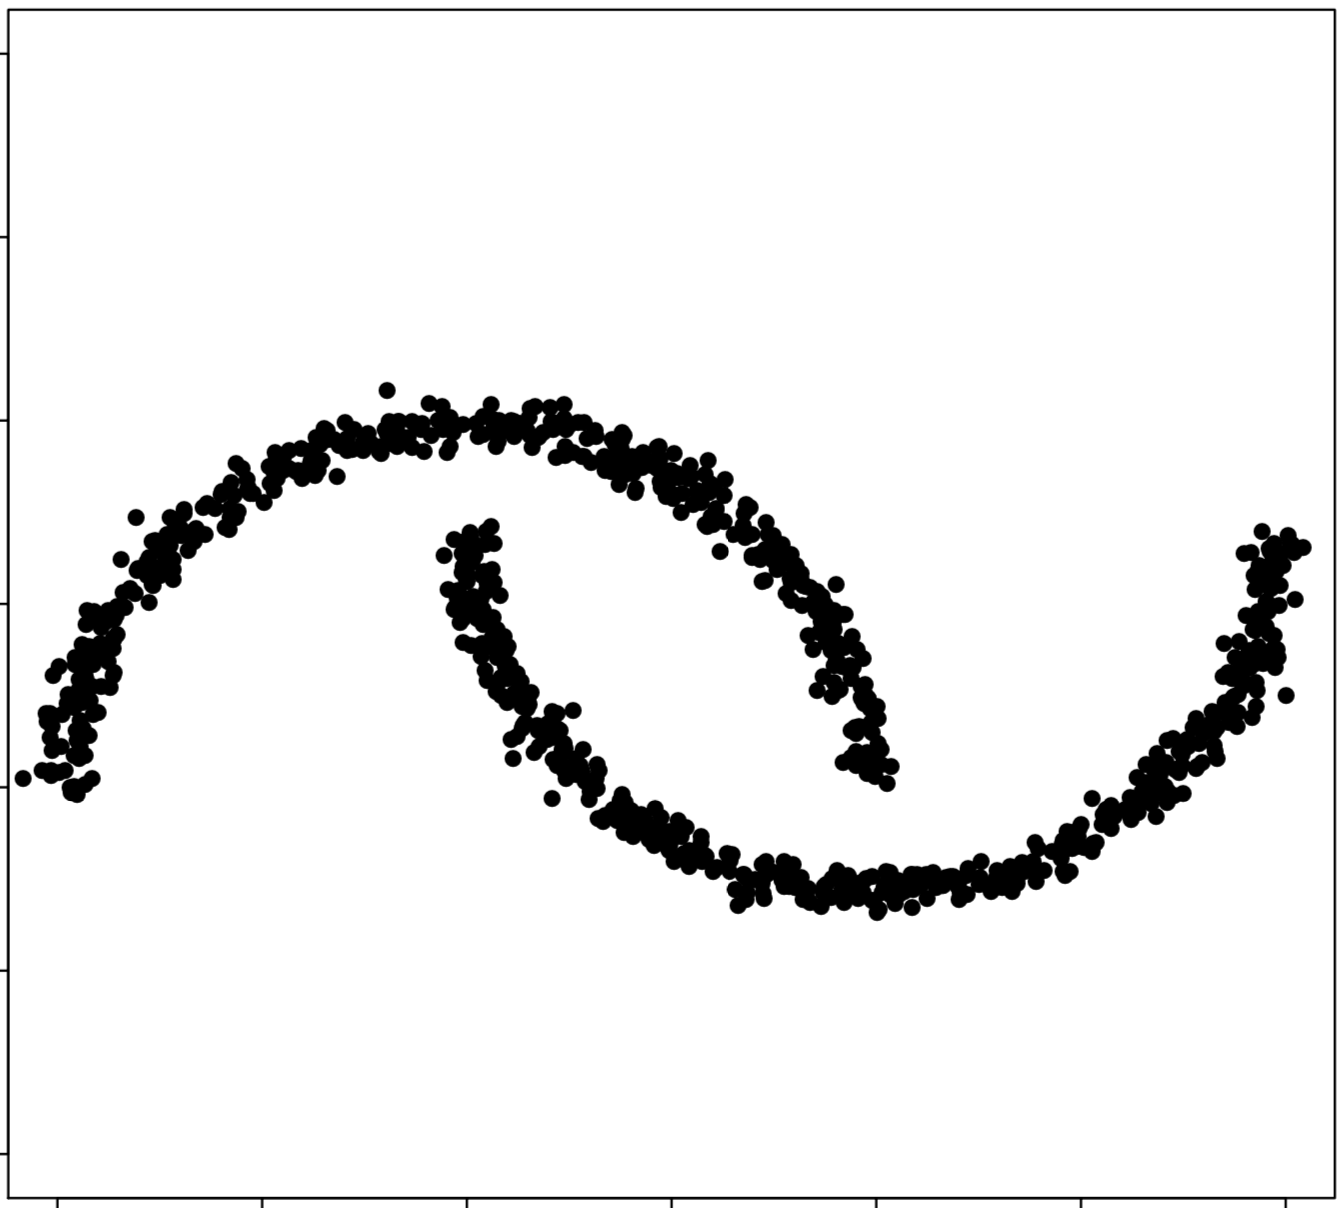
\includegraphics[width=6cm]{a2_hierarchy_1.png}
         \caption{ }
         \label{fig:moon}
     \end{subfigure}
        \hspace{5mm}
     \begin{subfigure}[b]{0.3\textwidth}
       %  \centering
    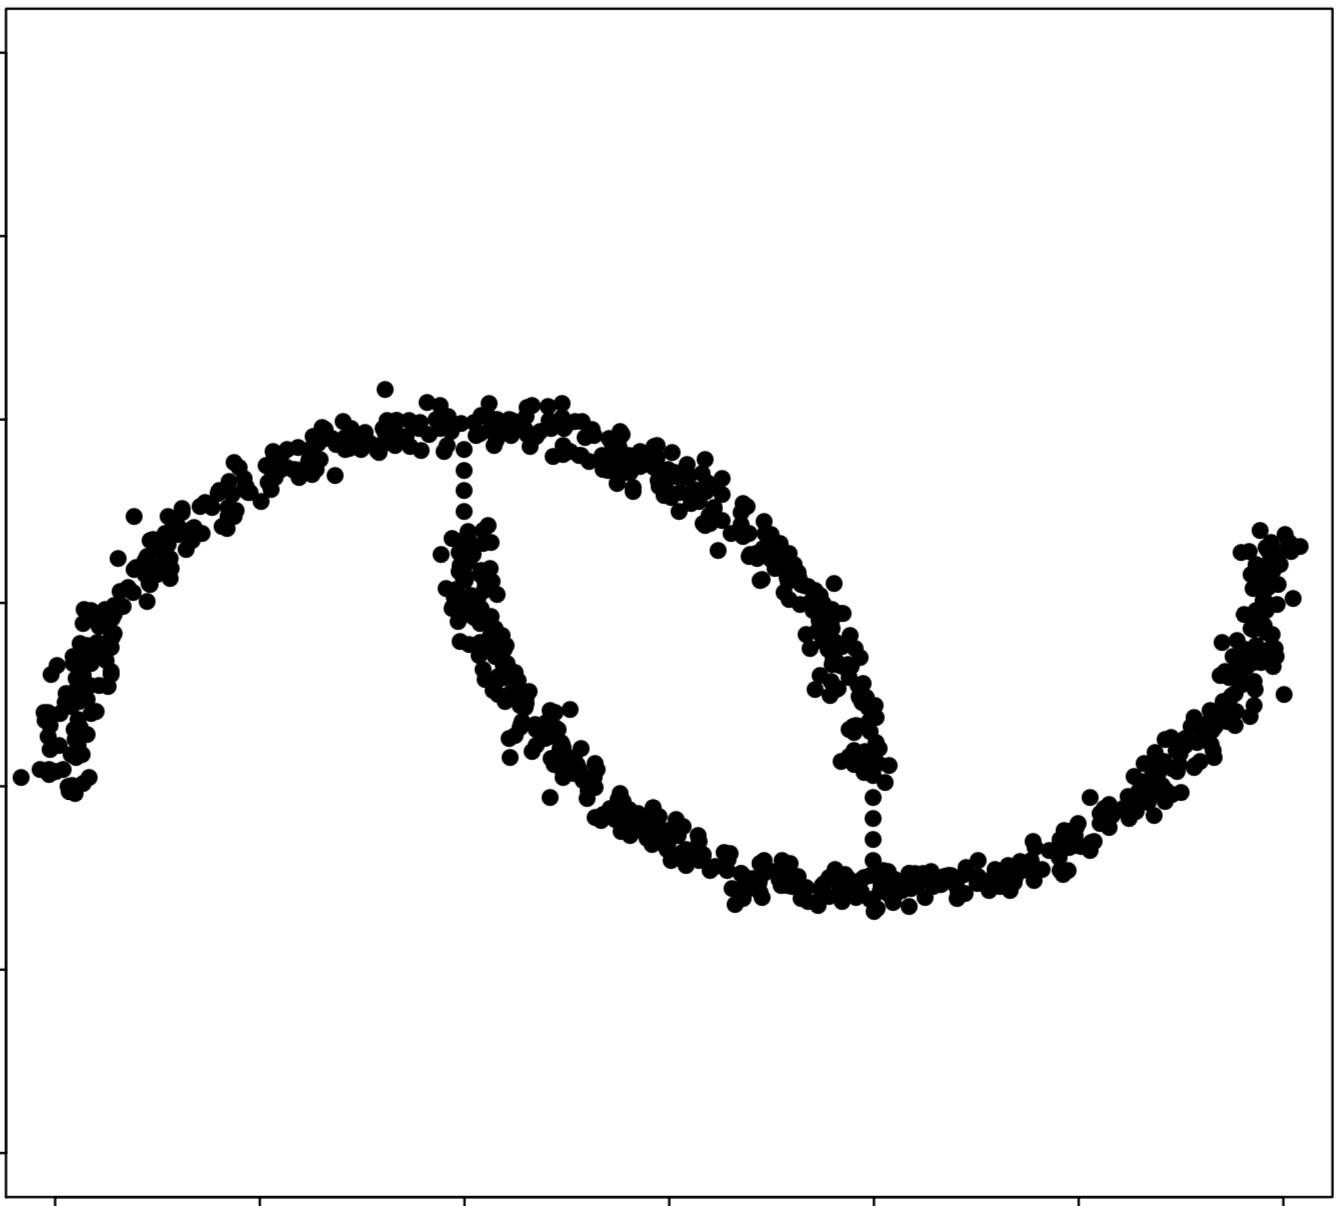
\includegraphics[width=6cm]{a2_hierarchy_2.png}
         \caption{ }
         \label{fig:joined_moon}
     \end{subfigure}
     \caption{(a) Standard moon crescent distribution. (b) Moon crescent distribution with data points in adjoining area.}
\label{fig:fig_hierarchy}
\end{figure}
\begin{solution}
\end{solution}

\part[3] Consider the distance matrix in Table \ref{fig:distance}. Show the hierarchy of  clusters created by the minimum distance hierarchical clustering algorithm, along with the intermediate steps. Finally, draw the dendrogram with edge lengths indicated.\\ 
(Note: You can draw the dendrogram on paper and upload the screenshot.)
\begin{table}[ht]
\caption{Distance between nodes} 
\label{fig:distance}
\centering 
\begin{tabular}{c c c c c c c} 
\hline\hline %inserts double horizontal lines
 & A & B & C & D & E \\ [0.5ex] % inserts table
%heading
\hline % inserts single horizontal line
A & 0 & 0.73 & 6.65 & 4.61 & 5.24  \\
B & 0.73 & 0 & 4.95 & 2.90 & 3.45  \\
C & 6.65 & 4.95 & 0 & 2.24 & 1.41  \\
D & 4.61 & 2.90 & 2.24 & 0 & 1  \\
E & 5.24 & 3.45 &1.41 & 1 & 0 \\
\hline 
\end{tabular}
\label{table:nonlin} % is used to refer this table in the text
\end{table}
\begin{solution}
\end{solution}

\part[2] Which distance metric (minimum, maximum and average) is more likely to generate following results given in Figure \ref{fig:cluster} for $K=2$? Why?\\
\begin{figure}[H]  
     \centering
     \begin{subfigure}[b]{0.3\textwidth}
         %\centering
    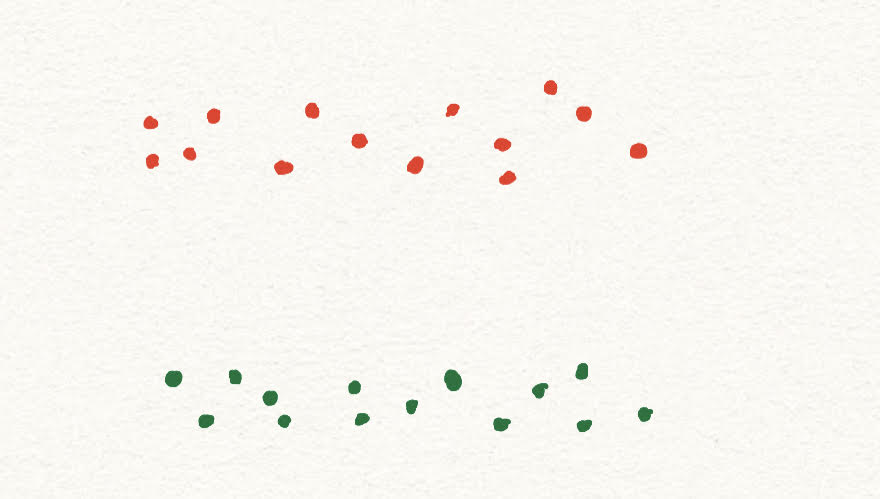
\includegraphics[width=6cm]{clusters.jpg}
         \caption{ }
     \label{fig:cluster}
     \end{subfigure}
     \caption{Result produced for $K=2$ clusters. Red points belong to one cluster and green to the other.}
\end{figure}
\begin{solution}
\end{solution}
\end{parts}


\question[10][{\sc Cutting Spectral apart}] One of the several ways to express a given dataset is by using a $\textit{graph}$. Each of the $N$ datapoints in the dataset can be thought of as a vertex/node in a graph and any two datapoints can be connected in the graph with an edge whose non-negative weight $W_{ij}$ indicates the similarity between the $i$th and $j$th datapoints. We will look at methods to partition this graph into two clusters, especially one that gained early prominence in computer vision. These methods can be recursively applied to partition the graph into any required number of clusters.
\begin{parts}
\part[1] A graph cut is a technique that separates a given graph into two disjoint sets of vertices and the degree of similarity (formally called the \textit{cut cost}) between the two sets is given by the sum of weights of the edges between the sets (i.e., edges whose two endpoint nodes lie in different sides of the partition). The obvious method to separate the data into two is by choosing a partition that has the minimum cut cost. What do you think is/are the drawback(s) of this method? (Hint: Think about the sizes of the two sets in the partition.)
\begin{solution}
\end{solution}

\part[2] Due to the above drawback(s), we use a variation of the min cut method called normalized cut to partition the graph into two. The problem of finding the minimum-cost normalized cut can be reduced to this problem:
\[
\centerline{$\textit{min}_{y}\frac{y^T(D-W)y}{y^TDy}$ subject to $y \in \{1, -c\}^N$ and $ y^TD\mathbf{1} = 0$}
\]
where $y_i$ takes one of the two discrete values $\{1, -c\}$ to indicate which side of the cut/partition the $i$th datapoint belongs to, $W$ is the symmetric $N \times N$ similarity (non-negative edge-weights) matrix, $D$ is a diagonal matrix called the degree matrix with $d_{ii} = \Sigma_{j}W_{ij}$, and $\mathbf{1}$ is a vector whose entries are all ones. This expression (not including the constraints) is called the $\textit{Generalized Rayleigh's Quotient}$ (GRQ). The matrix in the numerator, $D-W$ is the called the Laplacian Matrix, denoted by $L$. Prove that the Laplacian matrix is a singular matrix.
\begin{solution}
\end{solution}

\part[3] As the above minimization problem is NP-hard with the two constraints, we first let go of both constraints. Then, the above GRQ can be minimized over $y \in \mathbb{R}^N$ by solving the generalized eigenvalue system $(D-W)y = \lambda Dy$. Show that this equation can be expressed in the form $(ALA)z = \lambda z$, by expressing $A,z$ in terms of $D,W,y$. Compute the eigenvector corresponding to the smallest eigenvalue of the matrix $M = ALA$.
\begin{solution}
\end{solution}

\part[4] Now, let's bring back the constraint that $y^TD\mathbf{1}=0$ (the constraint that $y$ takes only two discrete values can remain relaxed as a final real-valued solution $\{y_i\}$ can be clustered using 2-means for instance to identify the desired partition). Prove that the GRQ above (subject to $y^TD\mathbf{1}=0$) is minimized when $y$ is the eigenvector corresponding to the second smallest eigenvalue of the generalized eigenvalue system $(D-W)y = \lambda Dy$. \\
(Hint: You can use the following fact. Let $A$ be a real symmetric matrix. Under the constraint that $x$ is orthogonal to the $(j-1)$ eigenvectors corresponding to the $(j-1)$ smallest eigenvalues of $A$, the Rayleigh's quotient $\frac{x^TAx}{x^Tx}$ is minimized when $x$ is the eigenvector corresponding to the $j^{th}$ smallest eigenvalue.)
\begin{solution}
\end{solution}
\end{parts}


\question[10] [{\sc Life in lower dimensions...}]
You are provided with a dataset of 1797 images in \href{https://drive.google.com/drive/folders/15msU-s48DApWteNbo9vNRXKAyid-HwwJ?usp=sharing}{a folder here} - each image is 8x8 pixels and provided as a feature vector of length 64. You will try your hands at transforming this dataset to a lower-dimensional space, and clustering the images in this reduced space. 

Please use the template .ipynb file in the \href{https://drive.google.com/drive/folders/15msU-s48DApWteNbo9vNRXKAyid-HwwJ?usp=sharing}{same folder} to prepare your solution. Provide your results/answers in the pdf file you upload to GradeScope, and submit your code separately in \href{https://courses.iitm.ac.in/mod/assign/view.php?id=78101}{this} moodle link. The code submitted should be a rollno.zip file containing two files: rollno.ipynb file (including your code as well as the exact same results/plots uploaded to Gradescope) and the associated rollno.py file.

\red{Write the code from scratch for both PCA and clustering. The only exception is the computation of eigenvalues and eigenvectors for which you could use the numpy in-bulit function.}

\begin{parts}
\part[3] Run PCA algorithm on the given dataset. Plot the cumulative percentage variance explained by the principal components. Report the number of principal components that contribute to 90\% of the variance in the dataset.
\begin{solution}
\end{solution}

\part[3] Perform reconstruction of data using the dimensionality-reduced data considering the number of dimensions [2,4,8,16]. Report the Mean Square Error (MSE) between the original data and reconstructed data, and interpret the optimal dimension $\widehat{d}$ based on the MSE values.
\begin{solution}
\end{solution}

\part[3] Apply K-means clustering on the reduced dataset from last subpart (b) (i.e., the $\mathbb{R}^{64}$ to $\mathbb{R}^\widehat{d}$ reduced dataset; pick the initial k points as cluster centers during initialization). Report the optimal choice of $K$ you have made from the set [1...15]. Which method did you choose to find the optimum number of clusters? And explain briefy why you chose that method. 

Also, show the 2D scatter plot (consider only the first two dimensions of optimal $\widehat{d}$) of the datapoints based on the cluster predicted by K-means (use different color for each cluster).
\begin{solution}
\end{solution}

\part[1] Summarise and explain your observations from the above experiments. Is the PCA+K-means clustering consistent with how your brain would cluster the images? 
\begin{solution}
\end{solution}
\end{parts}
\end{questions}
\end{document}

